\begin{enumerate}[label=\thesection.\arabic*.,ref=\thesection.\theenumi]
\numberwithin{equation}{enumi}

\item For a unity feedback system shown in Fig. 1
\begin{align}
G(s) =\frac{K}{s(s+2)(s+4)(s+6)}
\label{eq:ee18btech11036_system1}
\end{align}
Design a lead compensator to yield a $K_v$ = 2 and a phase margin of 30°.
\begin{figure}[!ht]
	\centering
	\resizebox{\columnwidth}{!}{%\begin{figure}
\tikzstyle{block} = [draw, fill=blue!20, rectangle, 
    minimum height=1cm, minimum width=1cm]
\tikzstyle{sum} = [draw, fill=blue!20, circle, node distance=1cm]
\tikzstyle{input} = [coordinate]
\tikzstyle{output} = [coordinate]
\tikzstyle{pinstyle} = [pin edge={to-,thin,black}]

% The block diagram code is probably more verbose than necessary
\begin{tikzpicture}[auto, node distance=2cm,>=latex']
    % We start by placing the blocks
    \node [input, name=input] {X(s)};
    \node [sum, right of=input] (sum) {};
    % \node [block, right of=sum] (controller) {k};
    \node [block, right of=sum] (system) {G(s)};
    % We draw an edge between the controller and system block to 
    % calculate the coordinate u. We need it to place the measurement block. 
    % \draw [->] (controller) -- node[name=u] {} (system);
    \node [output, right of=system] (output) {};
    \node [block, below of=system] (measurements) {1};

    % Once the nodes are placed, connecting them is easy. 
    \draw [draw,->] (input) -- node {$X(s)$} (sum);
    \draw [->] (sum) -- node {} (system);
    \draw [->] (system) -- node [name=y] {$Y(s)$}(output);
    \draw [->] (y) |- (measurements);
    \draw [->] (measurements) -| node[pos=0.99] {$-$} 
        node [near end] {} (sum);
\end{tikzpicture}
%\end{figure}
}
\caption{}
\label{fig:ee18btech11036}
\end{figure}

\solution 
For unity feedback we have Velocity error constant $\brak{K_v}$

\begin{align}
K_v &= \lim_{s \to 0} s G\brak{s} 
\label{eq:ee18btech11036_Kv}
\end{align}

\begin{align}
\lim_{s \to 0} \brak{\frac{K}{\brak{2+s}\brak{4+s}\brak{6+s}} }& = 2 
\\
\implies K = 96
\label{eq:ee18btech11036_init_cond}
\end{align}
Check the phase margin and gain crossover frequency by running the following code
\begin{lstlisting}
codes/ee18btech11036_1.py
\end{lstlisting}
\begin{itemize}
    \item The Phase margin: $19.76^{\circ}$
    \item Gain Crossover Frequency:1.469  rad/sec
\end{itemize}
The Bode plot of system is as shown,
\begin{figure}[!ht]
  \centering
  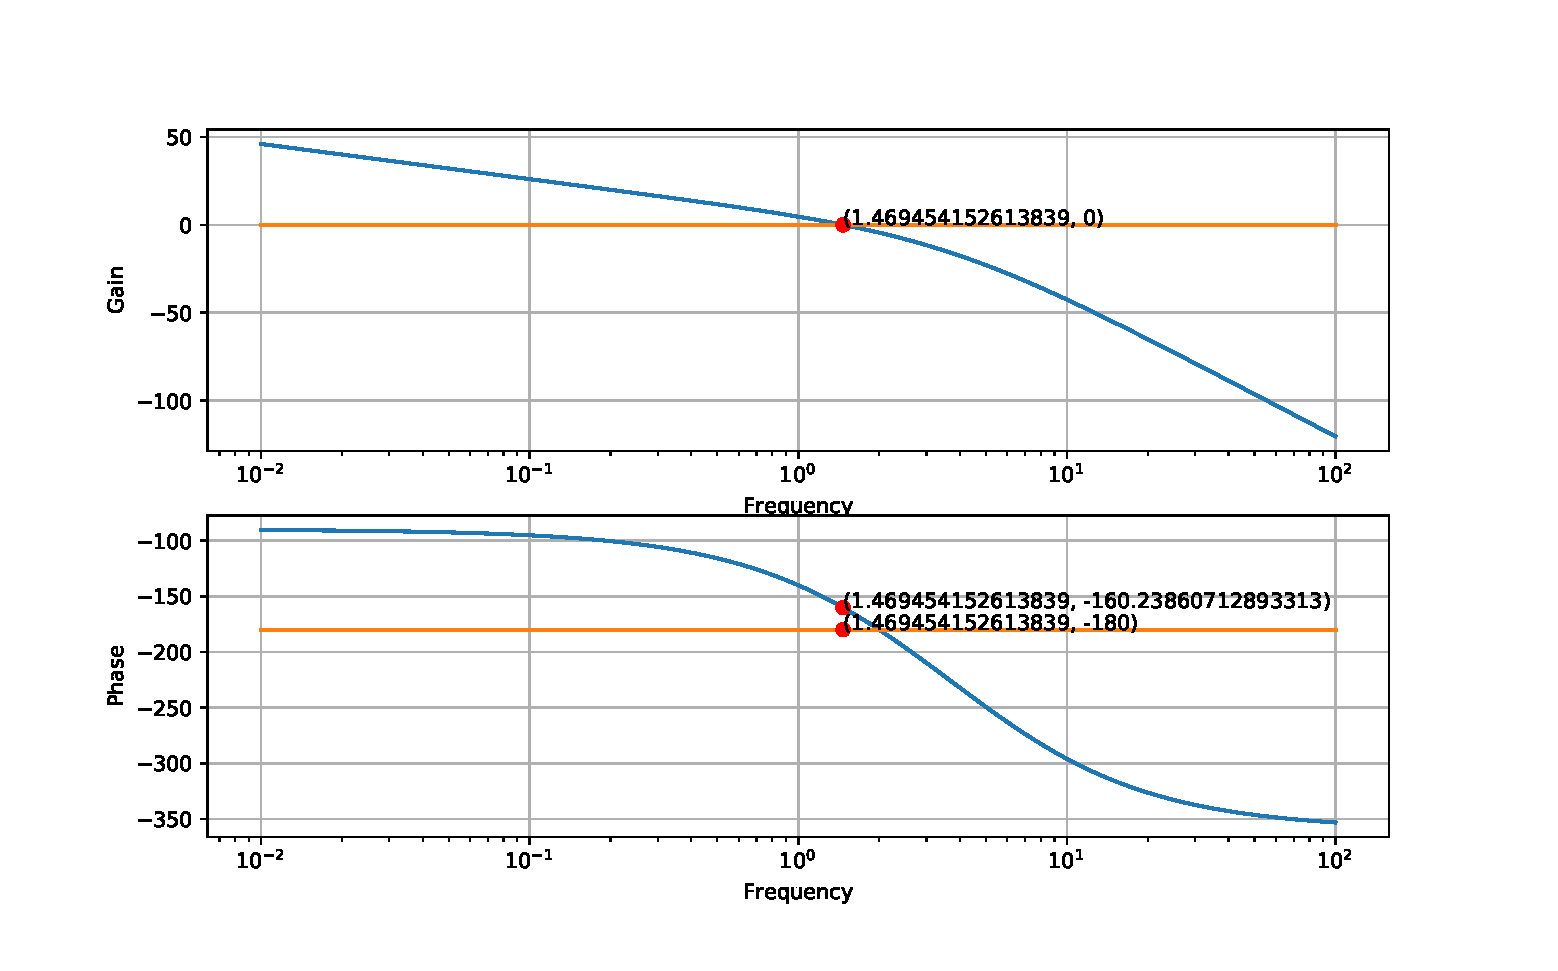
\includegraphics[width=\columnwidth]{./figs/ee18btech11036_1.eps}
  \caption{}
  \label{fig:ee18btech11036_1}
\end{figure}

Therefor amount of phase ot be added: 30-19.76=10.24





\item The circuit of lead compensator is given by
\begin{figure}[!ht]
    \centering
	\resizebox{\columnwidth}{!}{%\begin{figure}
\tikzstyle{block} = [draw, fill=blue!20, rectangle, 
    minimum height=1cm, minimum width=1cm]
\tikzstyle{sum} = [draw, fill=blue!20, circle, node distance=1cm]
\tikzstyle{input} = [coordinate]
\tikzstyle{output} = [coordinate]
\tikzstyle{pinstyle} = [pin edge={to-,thin,black}]

% The block diagram code is probably more verbose than necessary
\begin{tikzpicture}[scale=2]
    \draw[color=black, thick]
    (0,0) to (5,0){} 
    (0,2) to [short,-o] (0,1.5){}
    (0,0) to [short,-o] (0,0.5){}
    (0,1) node[]{\large{\textbf{INPUT}}}
    (0,2) to [R,l=$R_1$,](3,2)
    (0.7,3) to [C, l=$C$, *-] (2.3,3)
    (0.7,2) to (0.7,3){}
    (2.3,2) to (2.3,3){}
    (3,0) to [R,l=$R_2$,-*] (3,2)
    (3,2) to (5,2){}
    (5,2) to [short,-o] (5,1.5){}
    (5,0) to [short,-o] (5,0.5){} node[above=7mm]{\large{\textbf{OUTPUT}}}
    ;
\end{tikzpicture}
%\end{figure}

}
\caption{}
\label{fig:ee18btech11036_ckt}
\end{figure}

Transfer function:
\begin{align}
C(s)=\beta\brak{\frac{1+j\tau\omega}{1+j\beta\tau\omega}}
\label{eq:ee18btech11036_compensator}
\end{align}

\begin{align}
\beta=\brak{\frac{R_2}{R_1+R_2}}\\
\tau =R_1C
\label{eq:ee18btech11036_values}
\end{align}
Find the values of $\beta$ and $\tau$\\
\solution The maximum phase lead compensated by a lead compensator is given by\\
\begin{align}
\phi={\sin}^{-1}\frac{1-\beta}{1+\beta}
\label{eq:ee18btech11036_beta}
\end{align}
at
\begin{align}
\omega =\frac{1}{\sqrt{\beta}\tau}
\label{eq:ee18btech11036_omega}
\end{align}

Now we know that from Gain crossover frequency
\begin{align}
\omega =1.469 rad/sec
\end{align}
and the phase margin to be added:
\begin{align}
\phi =10.24^{\circ}
\end{align}
But to compensate for the added magnitude of lead compensator, a correction factor of $10^{\circ}-20^{\circ}$
is added.Hence
\begin{align}
\phi =30.24^{\circ}
\implies \beta=0.33
\end{align}
From the bode plot $\omega$ is chosen at which gain of original system is
\begin{align}
-20\log\brak{1/\sqrt{\beta}}&=-4.81
\end{align}
\begin{figure}[!h]
  \centering
  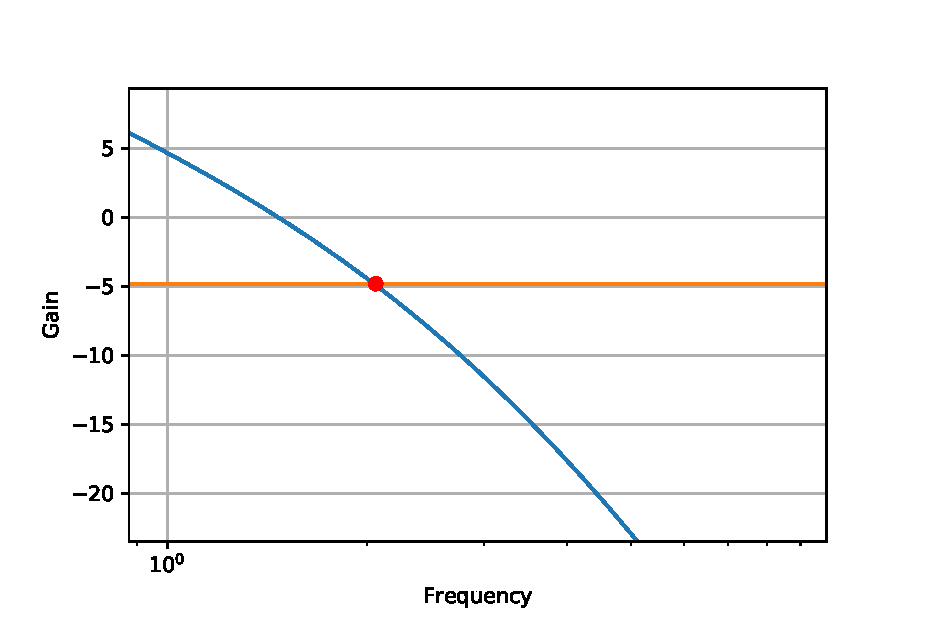
\includegraphics[width=\columnwidth]{./figs/ee18btech11036_3.eps}
  \caption{}
  \label{fig:ee18btech11036_3}
\end{figure}
Find the plot using the following code
\begin{lstlisting}
codes/ee18btech11036_4.py
\end{lstlisting}
From plot $\omega$=2.009 rad/sec\\
Solving equations \ref{eq:ee18btech11036_beta} and \ref{eq:ee18btech11036_omega}:
\begin{align}
\tau= 0.828\\
\beta=0.33\\
\label{eq:ee18btech11036_final}
\end{align}

New Transfer Function:
\begin{align}
G(s)=\frac{96\brak{1+ 0.828s}}{\brak{s}\brak{2+s}\brak{4+s}\brak{6+s}\brak{1+0.273s}}
\end{align}


\begin{figure}[!ht]
    \centering
	\resizebox{\columnwidth}{!}{%\begin{figure}
\tikzstyle{block} = [draw, fill=blue!20, rectangle, 
    minimum height=1cm, minimum width=1cm]
\tikzstyle{sum} = [draw, fill=blue!20, circle, node distance=1cm]
\tikzstyle{input} = [coordinate]
\tikzstyle{output} = [coordinate]
\tikzstyle{pinstyle} = [pin edge={to-,thin,black}]

% The block diagram code is probably more verbose than necessary
\begin{tikzpicture}[auto, node distance=2cm,>=latex']
    % We start by placing the blocks
    \node [input, name=input] {};
    \node [sum, right of=input] (sum) {};
    \node [block, right of=sum] (controller) {$ \beta(\frac{1+s\tau}{1+s\beta\tau})$};
    \node [block, right of=controller,
            node distance=3cm] (system) {$G(s)$};
    % We draw an edge between the controller and system block to 
    % calculate the coordinate u. We need it to place the measurement block. 
    \draw [->] (controller) -- node[name=u] {$U(s)$} (system);
    \node [output, right of=system] (output) {};
    \node [block, below of=u] (measurements) {1};

    % Once the nodes are placed, connecting them is easy. 
    \draw [draw,->] (input) -- node {$R(s)$} (sum);
    \draw [->] (sum) -- node {$E(s)$} (controller);
    \draw [->] (system) -- node [name=y] {$C(s)$}(output);
    \draw [->] (y) |- (measurements);
    \draw [->] (measurements) -| node[pos=0.99] {$-$} node [near end] {} (sum);
\end{tikzpicture}
%\end{figure}

}
\caption{}
\label{fig:ee18btech11036}
\end{figure}


\item
Verify your results from the following code:
\begin{lstlisting}
codes/ee18btech11036_2.py
\end{lstlisting}
\begin{itemize}
    \item The Phase margin: $29.269^{\circ}$
    \item The Gain Crossover Frequency: 2.02 rad/sec
\end{itemize}
%
The Bode plot is as shown,
\begin{figure}[!h]
  \centering
  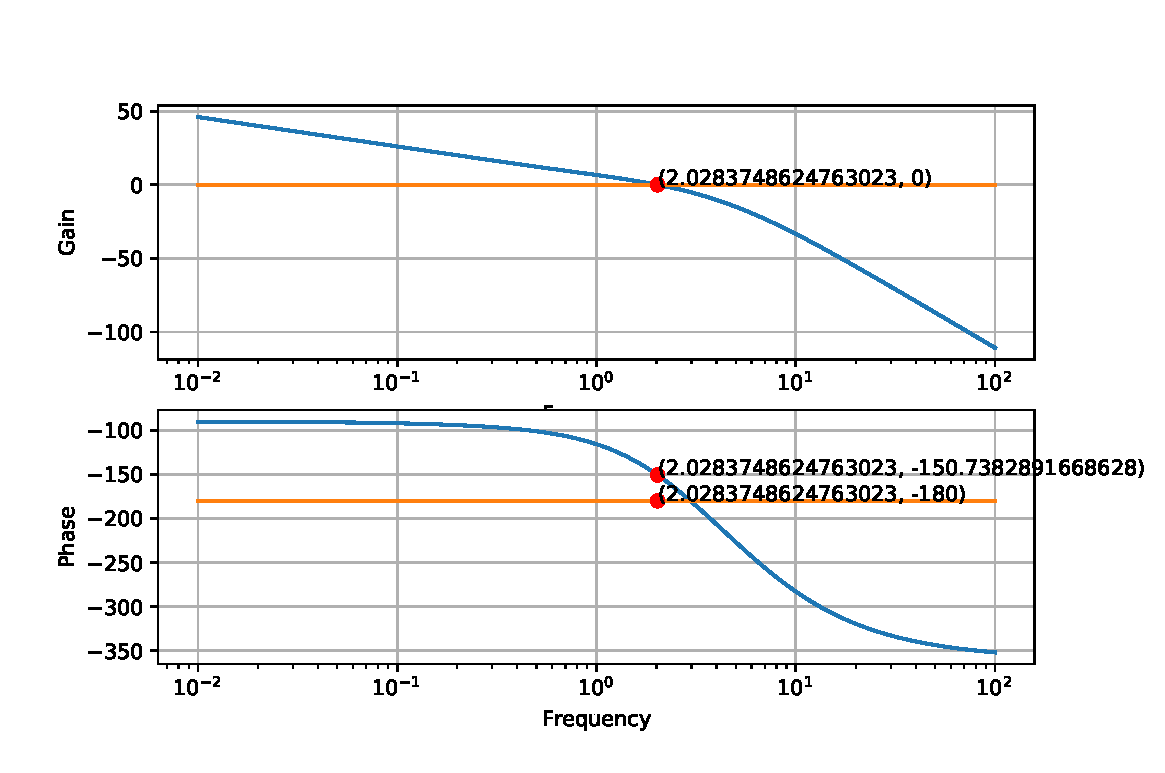
\includegraphics[width=\columnwidth]{./figs/ee18btech11036_2.eps}
  \caption{}
  \label{fig:ee18btech11036_2}
\end{figure}


\end{enumerate}
